%----------------------------------------------------------------------------------------
%	PACKAGES AND OTHER DOCUMENT CONFIGURATIONS
%----------------------------------------------------------------------------------------

\documentclass[a0paper,portrait]{baposter}

\usepackage[font=small,labelfont=bf]{caption} % Required for specifying captions to tables and figures
\usepackage{booktabs} % Horizontal rules in tables
\usepackage{relsize} % Used for making text smaller in some places

%\usepackage[utf8]{inputenc} % Polish language
%\usepackage{polski} % Polish language
%\usepackage[polish]{babel} % Polish language
\newcommand*\rot{\rotatebox{90}}
\usepackage{array,multirow,graphicx}
\usepackage{wrapfig} % Wrapping table
\usepackage{colortbl}% http://ctan.org/pkg/xcolor % Color cells

\usepackage{wrapfig} % Putting QR code
\usepackage{multicol} % Make 3 columns of itemized genomes groups

%\usepackage{graphics,graphicx} % POA graph example drawing
%\usepackage{pstricks,pst-node,pst-tree} % POA graph example drawing
\usepackage{tikz}

\usepackage{url}
\graphicspath{{images/}} % Directory in which figures are stored

\definecolor{bordercol}{HTML}{1b0d13} % Border color of content boxes
\definecolor{headercol1}{HTML}{582719} % Background color for the header in the content boxes (left side)
\definecolor{headercol2}{HTML}{a5694b} % Background color for the header in the content boxes (right side)
\definecolor{headerfontcol}{HTML}{e7dcc8} % Text color for the header text in the content boxes
\definecolor{boxcolor}{HTML}{e6e8ea} % Background color for the content in the content boxes

\begin{document}

\background{ % Set the background to an image (background.pdf)
\begin{tikzpicture}[remember picture,overlay]
\draw (current page.north west)+(-2em,2em) node[anchor=north west]
{
\includegraphics[height=1.1\textheight]{background}};
\end{tikzpicture}
}

\begin{poster}{
grid=false,
borderColor=bordercol, % Border color of content boxes
headerColorOne=headercol1, % Background color for the header in the content boxes (left side)
headerColorTwo=headercol2, % Background color for the header in the content boxes (right side)
headerFontColor=headerfontcol, % Text color for the header text in the content boxes
boxColorOne=boxcolor, % Background color for the content in the content boxes
headershape=roundedright, % Specify the rounded corner in the content box headers
headerfont=\Large\sf\bf, % Font modifiers for the text in the content box headers
textborder=rectangle,
background=user,
headerborder=open, % Change to closed for a line under the content box headers
boxshade=plain
}
{}
%
%----------------------------------------------------------------------------------------
%	TITLE AND AUTHOR NAME
%----------------------------------------------------------------------------------------
%
{\sf\bf Pan-genome structural analysis and visualisation} % Poster title
{\vspace{1em} Paulina Dziadkiewicz, Jakub Tyrek, Norbert Dojer\\ % Author names
{\smaller pedziadkiewicz@gmail.com, jakubtyrek@gmail.com, dojer@mimuw.edu.pl}} % Author email addresses
{
\includegraphics[scale=0.6]{english_logo}} % University/lab logo

%----------------------------------------------------------------------------------------
%	INTRODUCTION
%----------------------------------------------------------------------------------------

\headerbox{Introduction-OK}{name=introduction,column=0,row=0}{
Multiple sequence alignment is an information-rich object. Our aim is to analyze its component sequences by building a tree which consists of consensuses extracted from the alignment.\\ \\
A powerful way to achieve this result is to use graph representation of multiple alignment. It can be examined visually and be processed efficiently.
}

%----------------------------------------------------------------------------------------
%	GRAPH REPRESENTATION
%----------------------------------------------------------------------------------------

\headerbox{Graph Idea-OK}{name=graph,column=0,below=introduction}{

\begin{description}
\item[Graph representation] of multiple alignment is based on partial order alignment graph\cite{lee02}. It reflects the multiple alignment structure in a more concise and intuitive way than typical approaches like MAF files or alignment browsers.
\end{description}
The basic idea is to merge aligned nucleotides which are the same into single nodes, create directed edges between subsequent nodes and undirected edges between aligned but different nucleotides.
\begin{center}
\texttt{CATCGATGA} \\
\texttt{GATG-TTGA} 
$$\downarrow$$
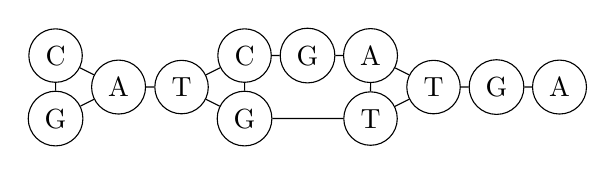
\begin{tikzpicture}
  [scale=.4,auto=left,every node/.style={circle,draw}]
  \node (n1) at (1,10) {C};
  \node (n2) at (1, 8) {G};
  \node (n3) at (3, 9) {A};
  \node (n4) at (5, 9) {T};
  \node (n5) at (7,10) {C};
  \node (n6) at (7, 8) {G};
  \node (n7) at (9,10) {G};
  \node (n8) at (11,10){A};
  \node (n9) at (11,8) {T};
  \node (n10) at (13,9) {T};
  \node (n11) at (15,9) {G};
  \node (n12) at (17,9) {A};
  
  \draw (n1) -> (n3);
  \draw (n2) -> (n3);
  \draw (n3) -> (n4);
  \draw (n4) -> (n5);
  \draw (n4) -> (n6);
  \draw (n5) -> (n7);
  \draw (n7) -> (n8);
  \draw (n6) -> (n9);
  \draw (n8) -> (n10);
  \draw (n9) -> (n10);  
  \draw (n10) -> (n11);
  \draw (n11) -> (n12);
  \draw (n1) -> (n2) [dashed];
  \draw (n5) -> (n6) [dashed];
  \draw (n8) -> (n9) [dashed];

\end{tikzpicture}
\end{center}

\begin{description}
\item[Consensuses] can be find in such a graph by using heaviest bundle algorithm implemented in software called \textsl{poa}\cite{lee04}. It reads the POA graph and effectively finds possible consensuses.
\end{description}

}

%----------------------------------------------------------------------------------------
%	FUTURE WORK
%----------------------------------------------------------------------------------------

\headerbox{Future Work-OK}{name=conclusion,column=0,below=graph}{
\begin{description}
\item[Visualisation:] Development of the graph visualisation, especially to make it more interactive.
\end{description}
\begin{description}
\item[Import/Export:] More formats of input and output files will be introduced in order to assure broad software compatibility.
\end{description}
\begin{description}
\item[Algorithms:] Development of fast algorithm for handling cycles in genome graphs.
\end{description}
}

%----------------------------------------------------------------------------------------
%	REFERENCES
%----------------------------------------------------------------------------------------

\headerbox{References-OK}{name=references,column=0,below=conclusion}{

\smaller % Reduce the font size in this block

\renewcommand{\section}[2]{} % Get rid of the default "References" section title
\begin{thebibliography}{1}
\bibitem{lee02}
  Lee C., Grasso C., Sharlow M.F.
  \textit{Multiple sequence alignment using partial order graphs},
  Bioinformatics (2002) 18 (3): 452-464.
  
\bibitem{lee04}
  Lee C.
  \textit{Generating consensus sequences from partial order multiple sequence alignment graphs},
  Bioinformatics. (2003) 22;19(8):999-1008.
  
\bibitem{ebolaportal}
Haeussler et al. 
\textit{The UCSC Ebola Genome Portal.},
 PLOS Currents Outbreaks. 2014 Nov 7 . Edition 1. doi: 10.1371/currents.outbreaks.386ab0964ab4d6c8cb550bfb6071d822.

\bibitem{mycoplasma}
\textit{Mycoplasma genomes phylogeny} \url{https://www.patricbrc.org/view/Taxonomy/2093#view_tab=phylogeny}, Accessed: April 2018
\end{thebibliography}
}

%----------------------------------------------------------------------------------------
%	ACKNOWLEDGEMENTS
%----------------------------------------------------------------------------------------

\headerbox{Acknowledgements-OK}{name=acknowledgements,column=0,below=references, above=bottom}{
\smaller % Reduce the font size in this block
This work was supported by the National Science Centre, Poland, under grant number 2016/21/B/ST6/01471.} 


%----------------------------------------------------------------------------------------
%	METHODS AND DATA
%----------------------------------------------------------------------------------------

\headerbox{How to get the tree of consensuses?-OK}{name=methods,span=2,column=1,row=0}{ % To reduce this block to 1 column width, remove 'span=2'

Firstly, convert a multiple sequence alignment (eg. MAF file) into POA graph \textbf{G}. The consensuses tree is being built in a breadth first manner. In the following iterations, on the subsequent subgraphs \textbf{SG} of the original graph \textbf{G}, the procedure of consensus generation and sequences assignment is carried out:
\begin{center}
\begin{minipage}{0.49\linewidth}
\begin{enumerate}
\setlength\itemsep{0em}
\item Run consensus generation algorithm on the \textbf{SG} to get a consensus \textbf{C}
\item Choose the most compatible to \textbf{C} sequences from \textbf{SG} and generate a consensus \textbf{BestC} for them only.
\item Set group \textbf{S} of the most compatible to \textbf{BestC} sequences from the \textbf{SG}.
\item Add \textbf{BestC} with sequences \textbf{S} to the consensuses tree and assign the minimum compatibility among \textbf{S} to \textbf{BestC}.
\item Remove from \textbf{SG} sequences \textbf{S} and go to 2 if any sequences are left.
\end{enumerate}
\end{minipage}
\begin{minipage}{0.49\linewidth}
\begin{center}
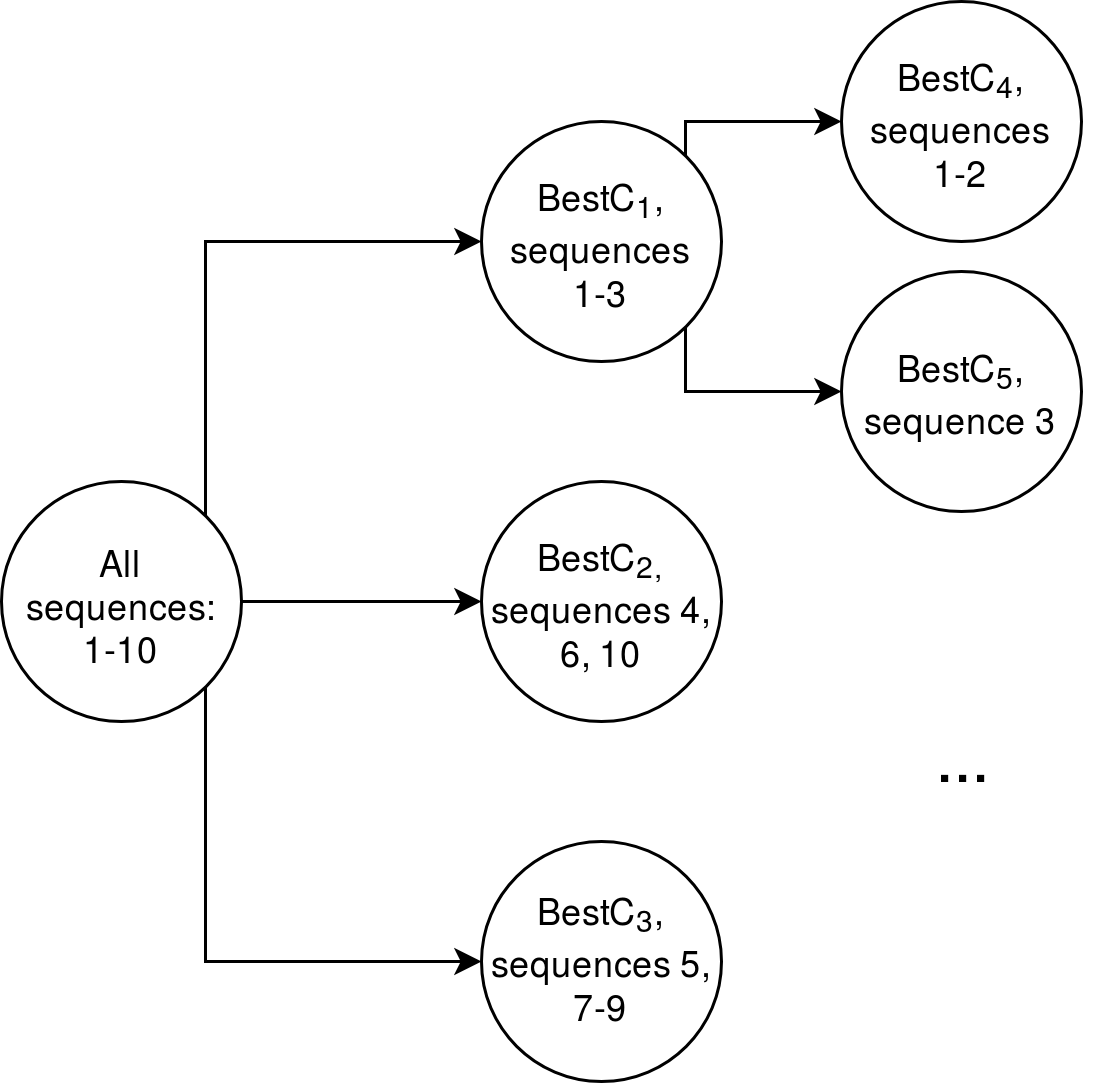
\includegraphics[scale=0.13]{consensuses_tree}
\captionof{figure}{Tree of consensuses}
\end{center}
\end{minipage}
\end{center}

Use the above schema to split group of sequences and assign a best consensus for them, until required level of fragmentation is reached.

%Data used in this research come from USCB Ebola Portal\cite{ebolaportal}. There is a multiple alignment (in MAF format) available,  generated from 158 Ebola and 2 Marburg viruses genomes coming from all over the world, which were sequenced at different times. The alignment has no cycles. According to the authors', the genomes can be split into 7 groups:
%\small{
%\begin{multicols}{3}
%\begin{itemize}
%\item Ebola 2014 (101)
%\item DRC 2007 (20)
%\item Zaire(DRC) 1967-7 (8)
%\item Bundibugyo 2007 (8)
%\item Reston 1989-90 (9)
%\item Sudan 1976 (11)
%\item Marburg 1987 (2)
%\end{itemize}
%\end{multicols}}
%
%\par In order to analyze this multiple alignment: generate consensuses, partition data into subsets and compare the division with the one discribed above, the available data must have been converted into POA graph and used as \textsl{poa}'s input. The output has been visualized and summarized in a readible manner.
%\begin{wrapfigure}{r}{0.1\textwidth}
%  \vspace{-20pt}
%  \begin{center}
%    
\includegraphics[width=0.07\textwidth]{qrcode}
%  \end{center}
%  \vspace{-40pt}
%  \hspace{-50pt}
%\end{wrapfigure}
%\par As a consequence of taking this approach, a tool for performing the above operations was developed. It is also possible to acquaint with some online results:
%
}

%----------------------------------------------------------------------------------------
%	RESULTS 1
%----------------------------------------------------------------------------------------

\headerbox{Single Alignment Block Analysis-TODO}{name=results1,span=2,column=1,below=methods}{ % To reduce this block to 1 column width, remove 'span=2'
An example block of the Ebola virus multiple alignment (ca. 3008 - 3200bp) can clearly demonstrate the multiple alignment visulisation and consensuses generation: 

%------------------------------------------------

\begin{center}
\begin{minipage}{0.49\linewidth}
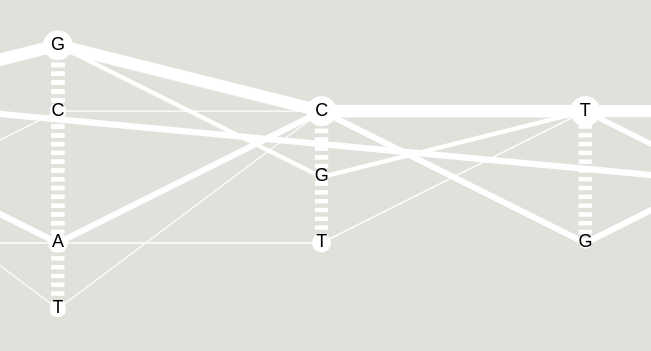
\includegraphics[width=1\linewidth]{ebola100_no_cons}
\captionof{figure}{Example POA graph fragment}
\end{minipage}
\begin{minipage}{0.49\linewidth}
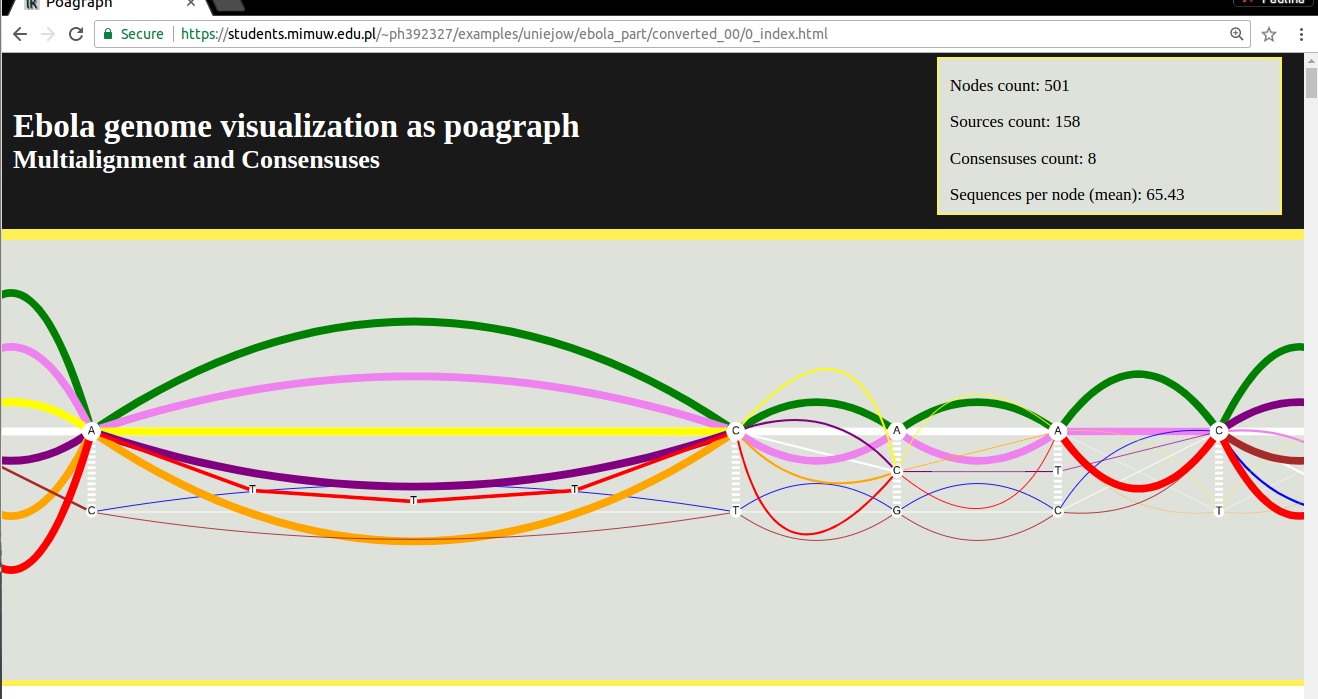
\includegraphics[width=1\linewidth]{ebola_part}
\captionof{figure}{Example with generated consensuses}
\end{minipage}
\end{center}

The tool output is not only the POA graph visualization (Fig.1) but also source sequences and generated consensuses summary (Fig.2). It is possible to assess, whether the original Ebola virus genomes clustering is common with the one being this method's result. 
}

%----------------------------------------------------------------------------------------


%----------------------------------------------------------------------------------------
%	RESULTS 2
%----------------------------------------------------------------------------------------

\headerbox{All Alignment Blocks Analysis-TODO}{name=results2,span=2,column=1,below=results1,above=bottom}{ % To reduce this block to 1 column width, remove 'span=2'
The above described approach applied to the whole Ebola virus multiple alignment resulted in 17 consensuses:\\

\begin{tabular}{l l | l l l l l l l l l l l l l l l l l }
									&	& \multicolumn{16}{c}{Consensuses ID} \\ 
	  								&											 & 0 & 1 & 2 & 3 & 4 & 5 & 6 & 7 & 8 & 9 & 10 & 11 & 12 & 13 & 14 & 15 & 16  \\  \cline{1-19}
	\multirow{7}{*}{\rot{Ebola groups}} 	& Ebola 2014 	& \cellcolor{blue!25}101 & 0 & 0 & 0 & 0 & 0 & 0 & 0 & 0 & 0 & 0  & 0  & 0  & 0  & 0  & 0  & 0\\
									& DRC 2007 		& 0 & 0 & \cellcolor{blue!25}9 & \cellcolor{blue!25}10 & 0 & 0 & 0 & 0 & 0 & 0 & 0  & 0  & 0  & 0  & 0  & 0  & \cellcolor{blue!25}1\\
									& Zaire (DRC) 	& 0 & \cellcolor{blue!25}8 & 0 & 0 & 0 & 0 & 0 & 0 & 0 & 0 & 0  & 0  & 0  & 0  & 0  & 0  & 0\\
									& Bundibugyo 	& 0 & 0 & 0 & 0 & 0 & 0 & 0 & \cellcolor{blue!25}4 & 0 & 0 & 0  & 0  & \cellcolor{blue!25}2  & \cellcolor{blue!25}2  & 0  & 0  & 0\\
									& Reston 1989-90& 0 & 0 & 0 & 0 & 0 & \cellcolor{blue!25}2 & \cellcolor{blue!25}2 & 0 & 0 & \cellcolor{blue!25}2 & 0  & \cellcolor{blue!25}3  & 0  & 0  & 0  & 0  & 0\\
									& Sudan 		& 0 & 0 & 0 & 0 & \cellcolor{blue!25}4 & 0 & 0 & 0 & \cellcolor{blue!25}3 & 0 & \cellcolor{blue!25}3  & 0  & 0  & 0  & 0  & 0  & \cellcolor{blue!25}1\\
									& Marburg 		& 0 & 0 & 0 & 0 & 0 & 0 & 0 & 0 & 0 & 0 & 0  & 0  & 0  & 0  & \cellcolor{blue!25}1  & \cellcolor{blue!25}1  & 0\\

\end{tabular}

%\caption{Confusion matrix}
%\end{wraptable} 
%\end{center}
As one can see, the sequences where quite correctly distinguished. However, some groups (e.g. ''DRC 2007'', ''Bundibugyo'')  were split into smaller groups. This uncovers heterogeneity inside the original groups. Here is the example ''DRC 2007'' and the dates of origin of its sequences which explains the received partition:
\begin{center}
\begin{tabular}{|l|l|l|l|l|l|}
\hline
\multicolumn{2}{|c}{Genomes from 2007} & \multicolumn{2}{|c|}{Genomes from ca. 1995} & \multicolumn{2}{c|}{Genome from 2002} \\ \hline
\multicolumn{1}{|c|}{Name}   & \multicolumn{1}{c|}{Cons. ID} & \multicolumn{1}{c|}{Name}  & \multicolumn{1}{c|}{Cons. ID}  & \multicolumn{1}{c|}{Name}  & \multicolumn{1}{c|}{Cons. ID} \\ \hline
Luebo43\_2007 &  2 &	1Mbie\_Gabon\_1996	& 	3  & Ilembe\_2002 & 16 		\\ \hline
Luebo5\_2007  &  2 &	Gabon\_1994			& 	3	& & \\ \hline
Luebo4\_2007  &  2 &	1Eko\_1996			& 	3	& & \\ \hline
Luebo9\_2007  &  2 &	1Oba\_Gabon\_1996	& 	3	& & \\ \hline
Luebo23\_2007 &  2 &	Zaire\_1995			& 	3	& & \\ \hline
Luebo1\_2007  &  2 &	13709Kikwit\_1995 	& 	3	& & \\ \hline
Luebo0\_2007  &  2 &	1Ikot\_Gabon\_1996 	& 	3	& & \\ \hline
034-KS\_2008  &  2 &	13625Kikwit\_1995 	& 	3	& & \\ \hline
M-M\_2007	  &  2 &	2Nza\_1996	 		& 	3	& & \\ \hline
			  &	   &	Kikwit\_1995	 	& 	3	& & \\ \hline
\end{tabular}
\end{center}

%Ilembe\_2002 & 16 \\ 
%\end{tabular}


%------------------------------------------------

%\begin{center}
%\begin{minipage}{0.49\linewidth}
%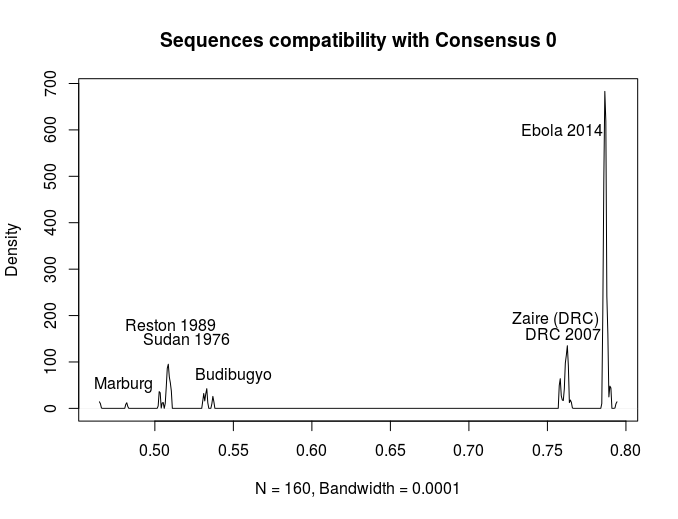
\includegraphics[width=0.9\linewidth]{Compatibility_CONS0}
%\end{minipage}
%\begin{minipage}{0.49\linewidth}
%By looking at the density plot of compatibility values, it is easy to notice that even if some sequences group were mapped to the same consensus ID, the distance between them and the consensus is different. The local maxima correspond, more or less, to the original genomes distribution.\\
%Combination of different analysis can result in accurate genomes partitioning and finding adequate consensuses.
%\end{minipage}
%\end{center}
%
%
%
}

\end{poster}

\end{document}
